\section{Simulation Architecture}

\begin{figure}[H]
    \centering
    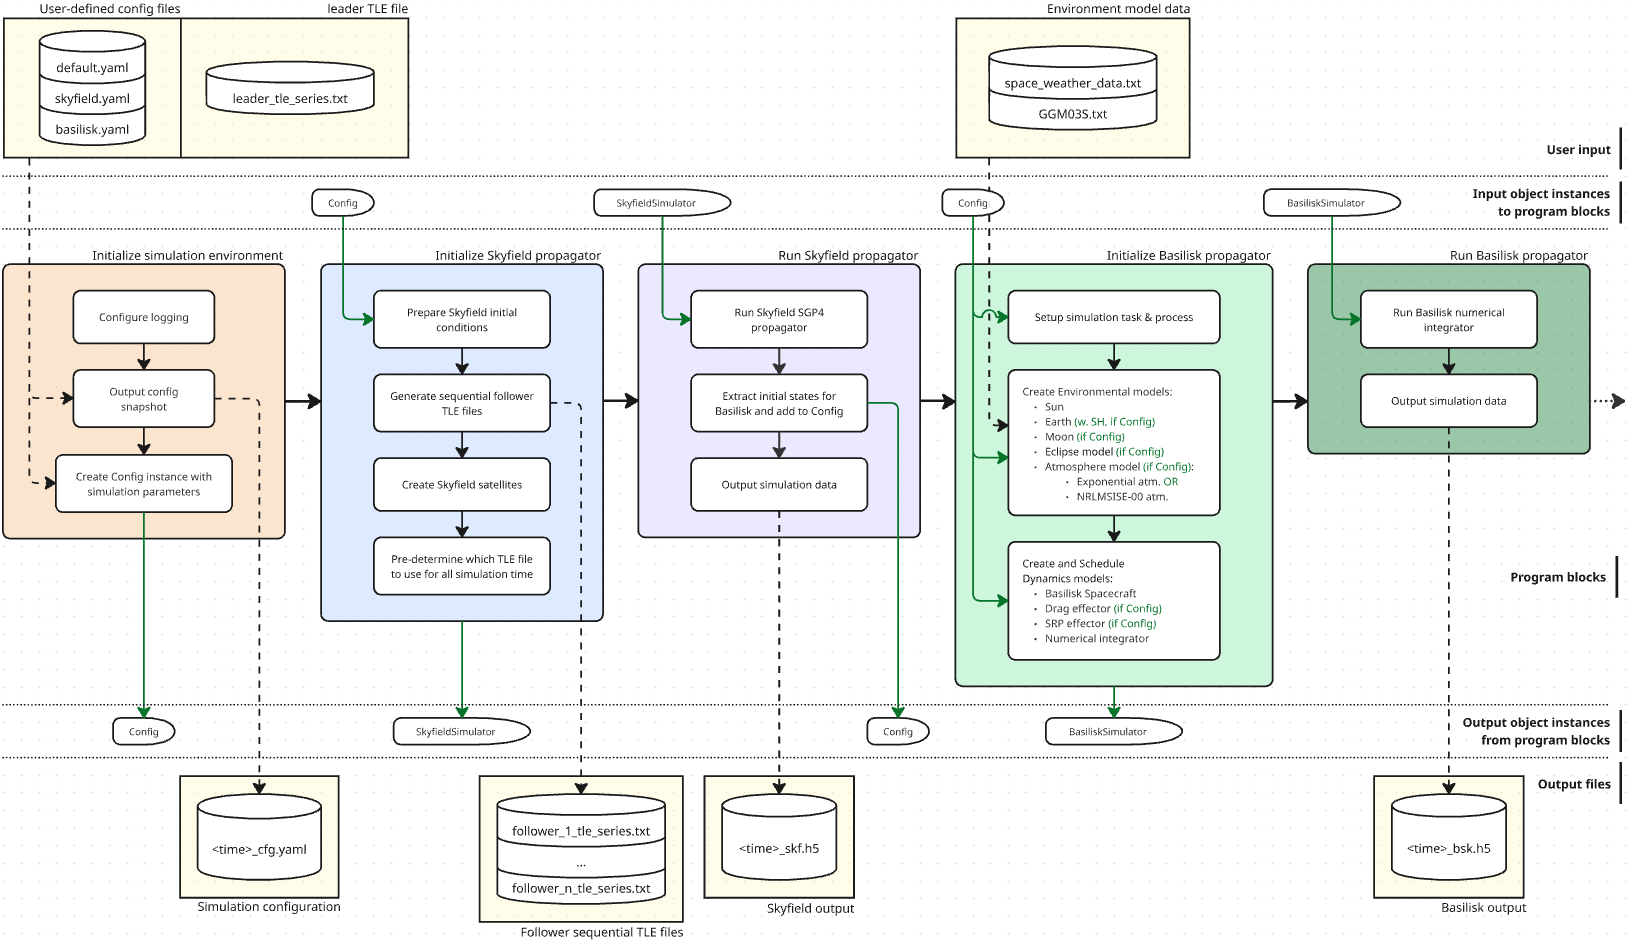
\includegraphics[width=1.0\textwidth]{Figures/04Method/Propagation Accuracy Comparison Simulator Flowchart.png}
    \caption{Adopted from \cite{hystad2025}}.
    \label{fig:propagator_comp_flow} 
\end{figure}


\section{Skyfield SGP4 Reference Methodology}
\begin{comment}
This section should present:
* TLE handling / follower generation
* Sequential TLE usage
* Why this is useful as a propagation comparison baseline
\end{comment}


\section{Propagation Initialization \& Execution}
\begin{comment}
Should present: (I am a bit unsure about this section => Subject to change. NOTE: Some of this might be better suited for the "Validation and Mission analysis methodology" chapter)
* The orbital configuration used (initial along-track spacing)
* Spacecraft configuration (reduced variant of the one presented earlier)
* Time horizon
\end{comment}

